\section{Conceptualization}
\label{sec:concept}

\subsection{Relevant Parameters}

A prioritization of elements is necessary for decisions on visual hierarchy, as well as which elements can be left out if there is not enough space.

\begin{table}[hb]
    \begin{tabular}{l | p{0.25\linewidth} | p{0.25\linewidth} | p{0.25\linewidth}}
        & Display Mode & Visualization \\
        \hline
        Oxygen & Continuous & Status Bar, Value \\
        Hazard Proximity & Pop-Up & Icon \\
        Warning Notification & Pop-Up & Billboard \\
        Working Time & Pop-Up, Continuous & Countdown \\
        Heart Rate & Continuous & Icon, Value, Trend \\
        Ambient Temperature & Continuous & Icon, Value, Trend \\
        Humidity & Continuous &  Icon, Value \\
        Checklist & Continuous & Line Highlight \\
        Tool Help & Pop-Up & Icon, Value \\
    \end{tabular}
    \caption{Parameters chosen for visualization, ordered from most to least important.}
\end{table}

maybe columns: frequency of checking,

Continuous means that the component will be displayed permanently. Parameters marked with pop-up will be displayed occasionally when relevant. 

\subsection{Components}

Following the previous guidelines, every element is designed for maximum clarity.

\subsubsection{Visualizing Oxygen Usage Through a Status Bar}

Since the oxygen value is the crucial factor whether or not to continue work, this is the component taking the spotlight. As the most critical parameter, this component will be visible in any version of the HUD. To check the current status as quickly as possible, the value will be visualized with a status bar.

Visualization helps to avoid mental math.

graphical vs text: status bar is understood faster than the number amount + unit

The first decision was the way to visualize the status bar. Mechanical pressure gauges with mechanical pointer show visual progress by default. 
According to \textcite{xiaVisualizingWristImpact2025}, bar charts outperform radial visualization.

\begin{figure}[hbt]
    \centering
    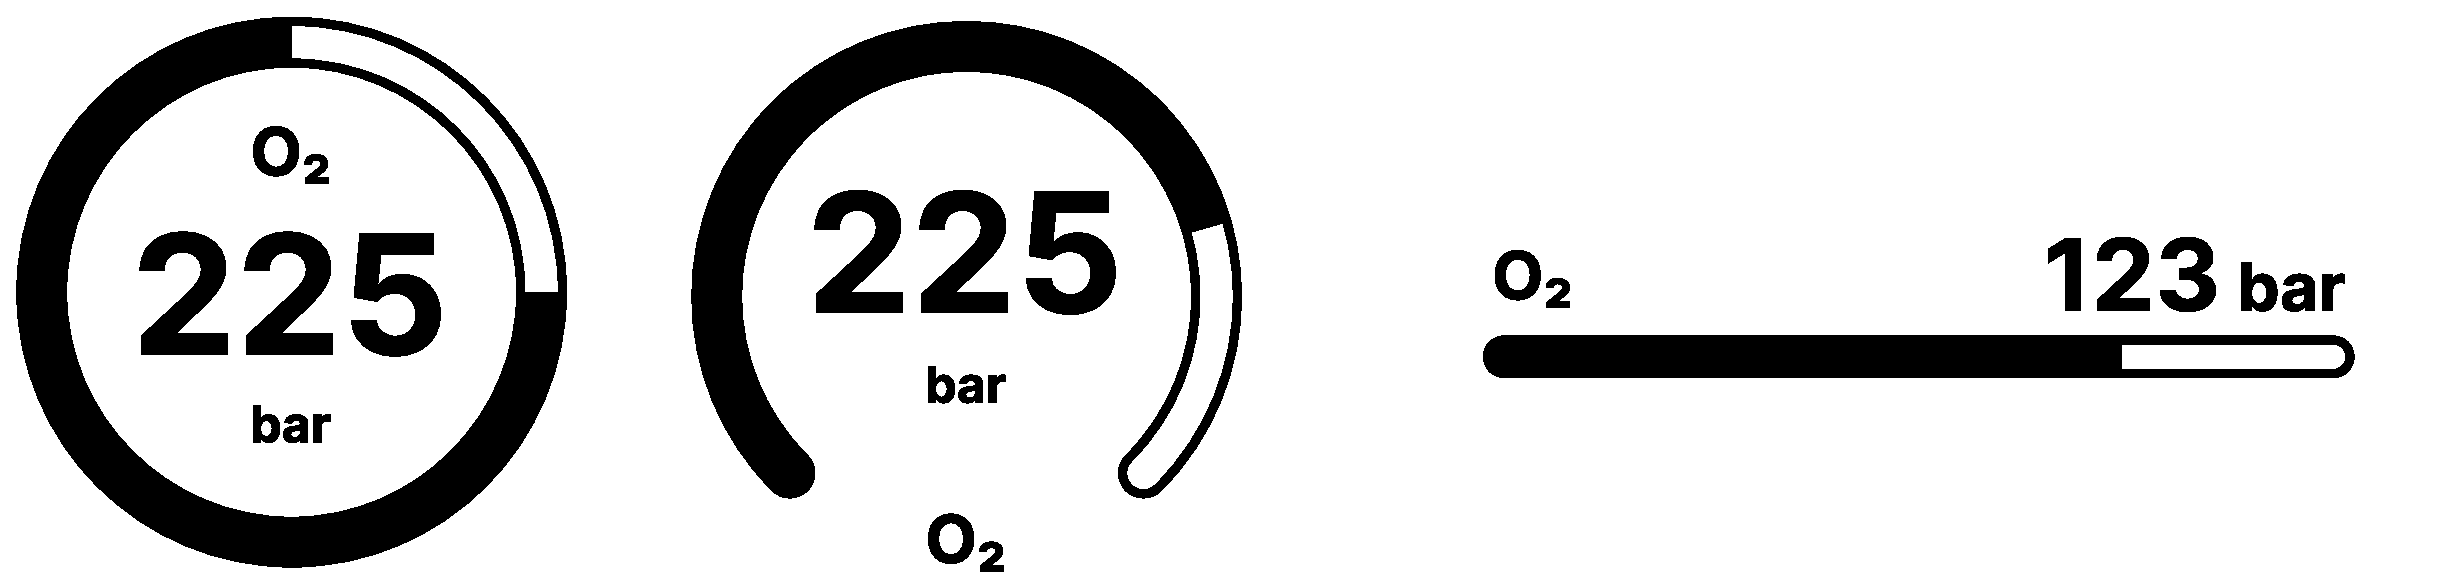
\includegraphics[width=1\textwidth]{assets/oxy_radial_bar.eps}
    \caption{The base component with configurable icon, parameter value, unit and trend indicator.}
    \label{fig:oxy_radial_bar}
\end{figure}

The second version implements the status bar in four segments, making it easier to estimate the amount left. Another hypothetical advantage of the gaps in the bar might be that more of the background can be seen.

\begin{figure}[hbt]
    \centering
    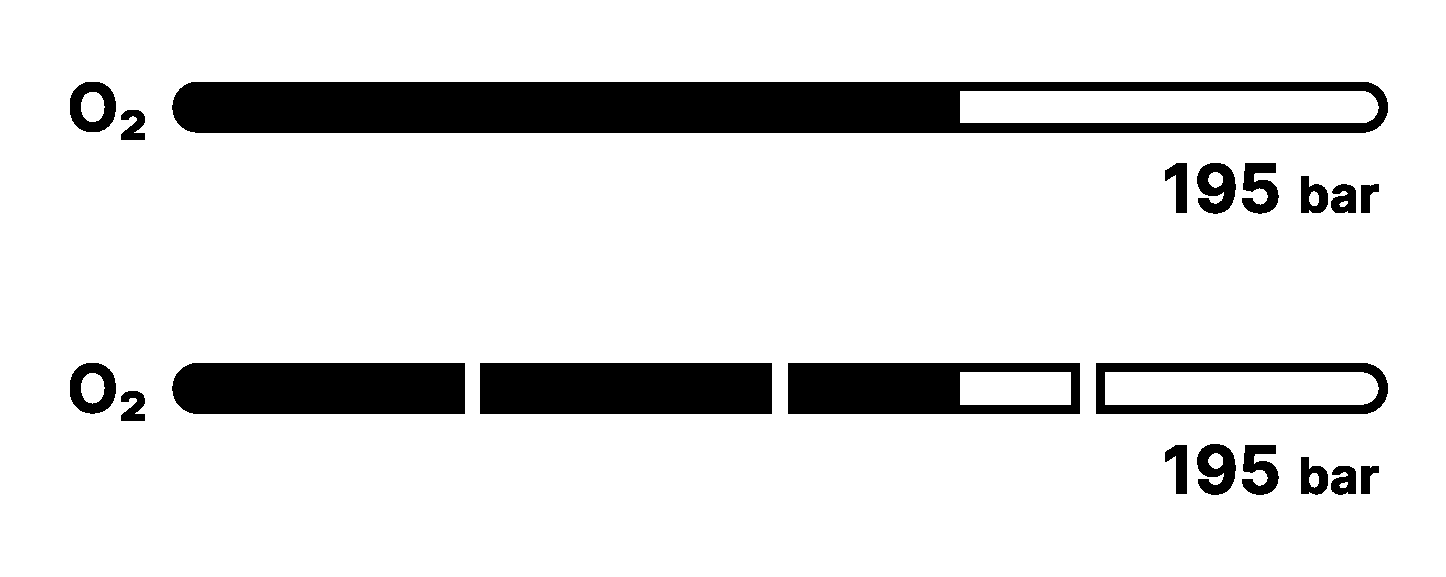
\includegraphics[width=1\textwidth]{assets/oxy_segment.eps}
    \caption{The base component with configurable icon, parameter value, unit and trend indicator.}
    \label{fig:oxy_segment}
\end{figure}

Depending on screen real estate, there are horizontal and vertical versions of the component.

In the horizontal version the label is placed in front of the bar so as not to have another "reading bump".

In the vertical orientation, the label and value are aligned at the top and bottom respectively, to account for visual crowding.

The oxygen value is located so that the status bar is seen first, e.g. if the component is on the left, the bar will be on the right side. This helps to maintain an optical guide.

- time left w/ current breathing rate

\begin{figure}[hbt]
    \centering
    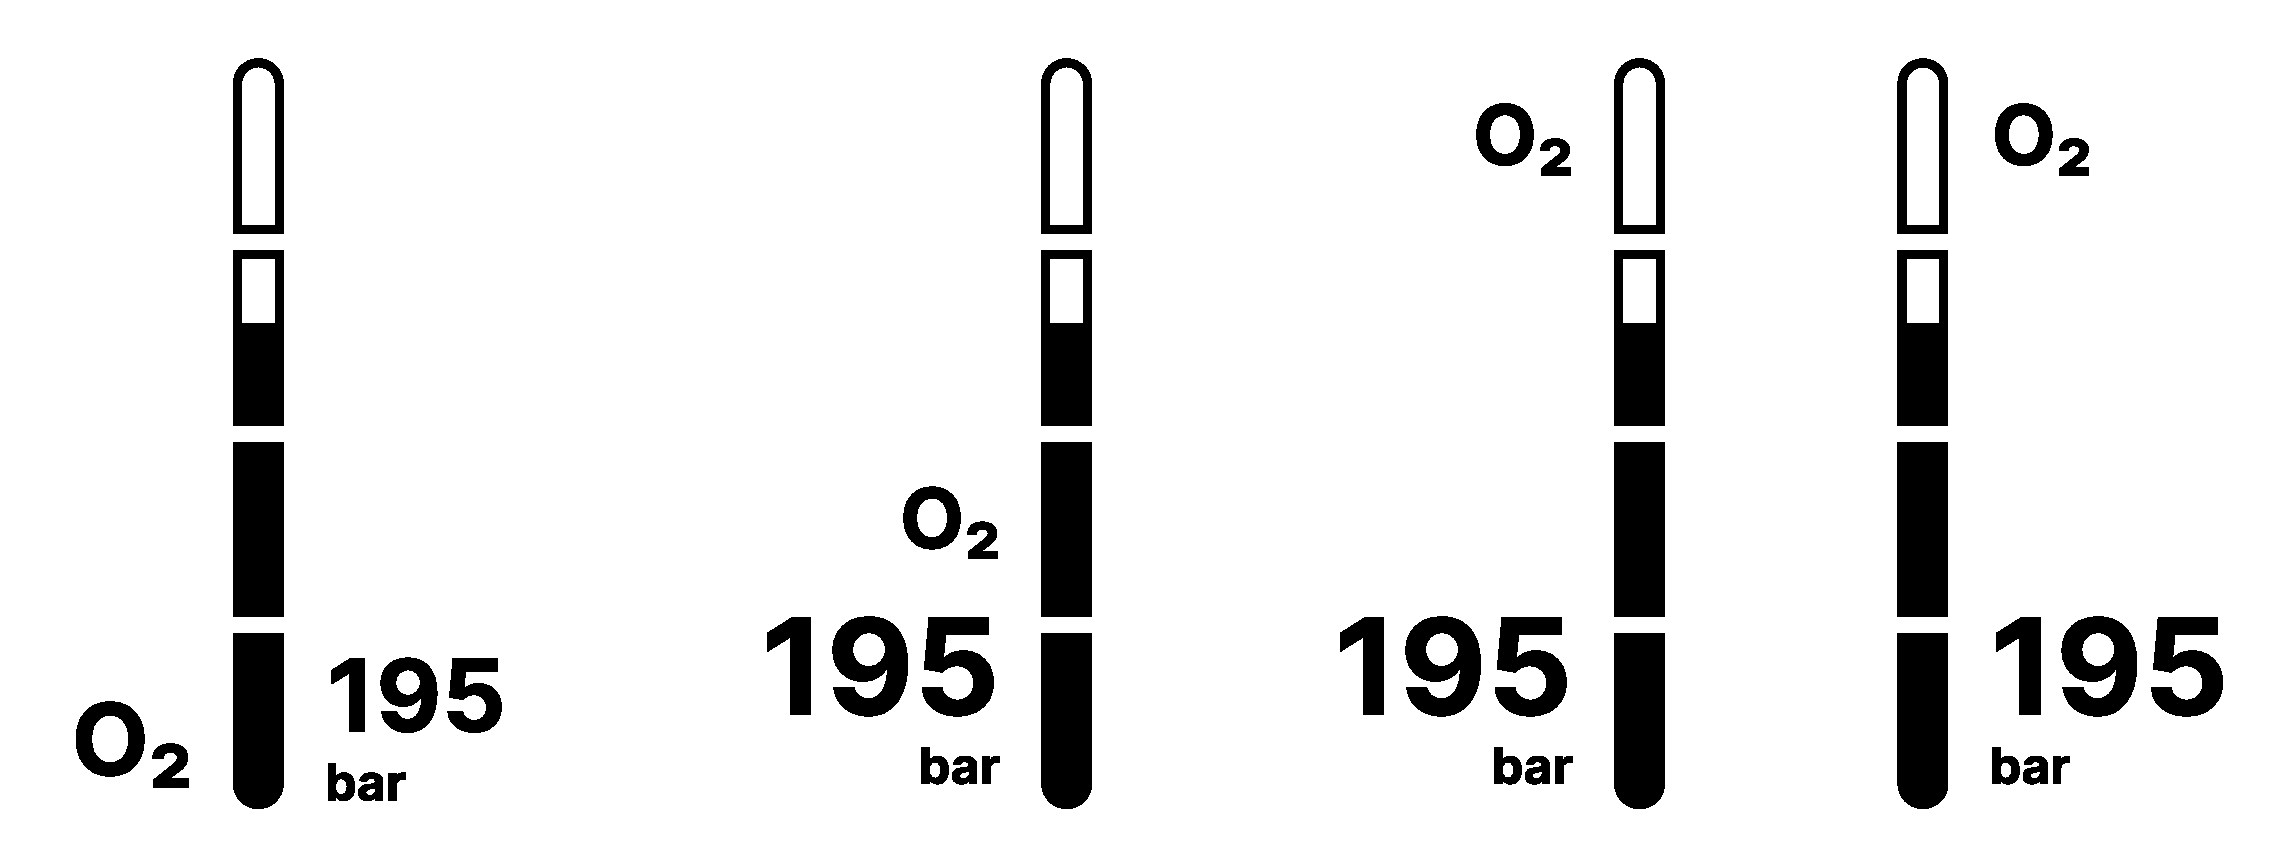
\includegraphics[width=1\textwidth]{assets/oxy_vertical.eps}
    \caption{The base component with configurable icon, parameter value, unit and trend indicator.}
    \label{fig:oxy_vertical}
\end{figure}

\subsubsection{The Base Component}

This element is built with a simple configuration for secondary information that is helpful but does not need to be prioritized. This includes factors like heart rate, but also environmental information such as ambient temperature or humidity.

Values that are not to be visualized are similar enough to be based on a universal base component. Apart from the actual parameter value, any of these elements can be hidden. This allows flexible configuration depending on the type of information.

The icons replace labels, and should therfore be as unambiguous as possible.
If the icon is unambiguous enough, it is easier to hide the unit. In some cases, the unit supports the identification of the value. Leaving the unit out saves space as well.

The trend indicators are displayed based on the difference of the current and previous value. If the value rises or falls an unusual amount, which could note environmental events. For dynamic elements like these, the frequency of changes should not be too high to avoid distraction.

Comparing the short and long arrows, the long arrows are better readable when out of focus.

\begin{figure}[hbt]
    \centering
    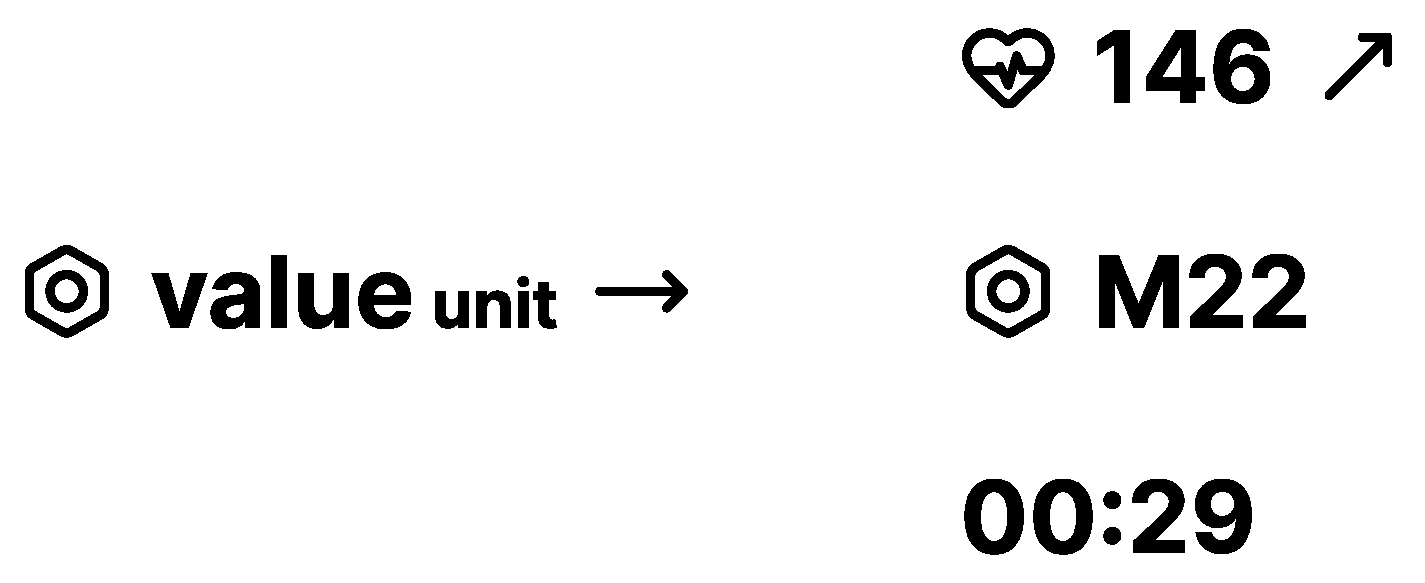
\includegraphics[width=1\textwidth]{assets/base_component.eps}
    \caption{The base component with configurable icon, parameter value, unit and trend indicator.}
    \label{fig:base_component}
\end{figure}

\begin{figure}[hbt]
    \centering
    %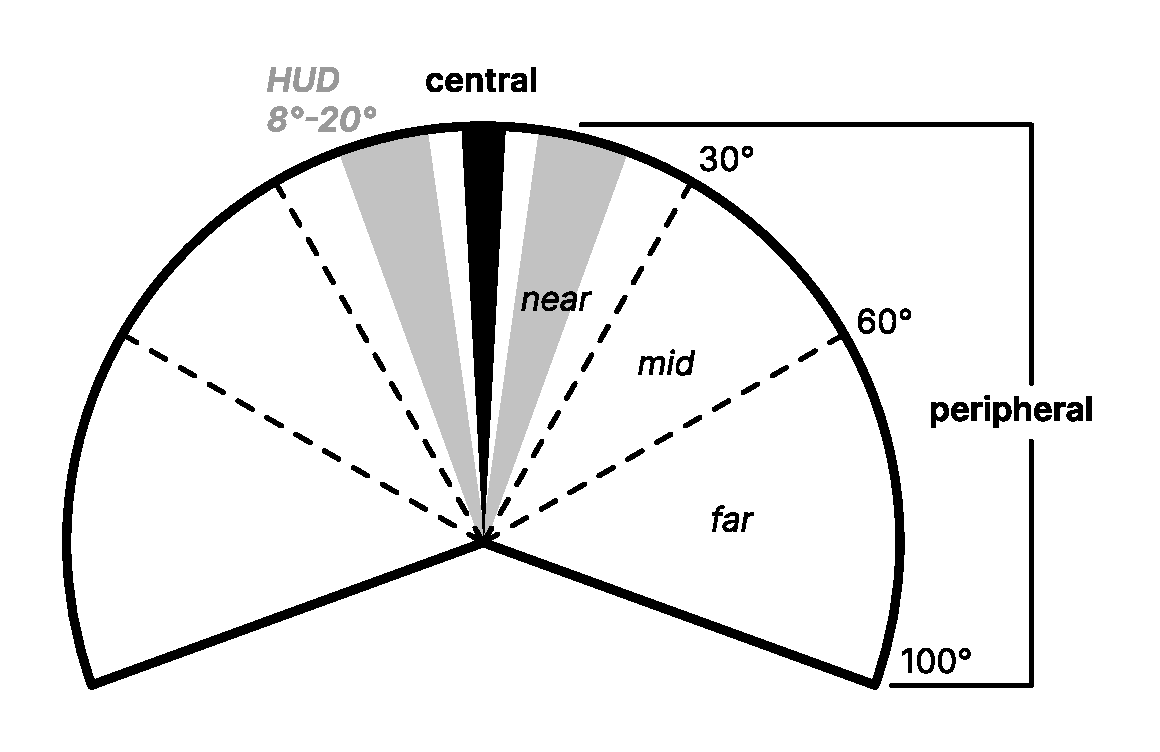
\includegraphics[width=0.5\textwidth]{assets/FOV.eps}
    \caption{Example configuration of the base component. Left to right: heart rate, time and tool help.}
    \label{fig:base_configs}
\end{figure}

The time component is a special case: it will only be displayed after a configured amount of time. The element popping up is meant to be perceivable in the peripheral vision, marking (for example) the halfway point. This action alone is therefore meaningful. Afterwards it can be checked consciously.

Since working time is limited by various parameters and therefore not fixed, it is a countdown. To avoid pulling unnecessary attention, the display is limited to minutes, instead of ticking down by the second.

\subsubsection{Notifications and Pop-Ups}

Instead of unique silhouettes, the hazard warnings are triangular to be more intuitive. The placement is therefore more important for peripheral distinction.
Both icons are placed close together so that they are visible at the same angle if multiple hazards are present. Similar to a car's dashboard warning lights, each of them has a fixed position, facilitating quicker information acquisition. With regular notifications—depending on which appeared first—the order of content would be different.

Horizontal versus vertical arrangement
Since the visual search field is wider than it is tall, 
horizontal might blend together, stacked vertically—therefore at the same visual angle—they might be more distinctive. More a loose guideline, flexible in regard to screen real estate.

\begin{figure}[hbt]
    \centering
    %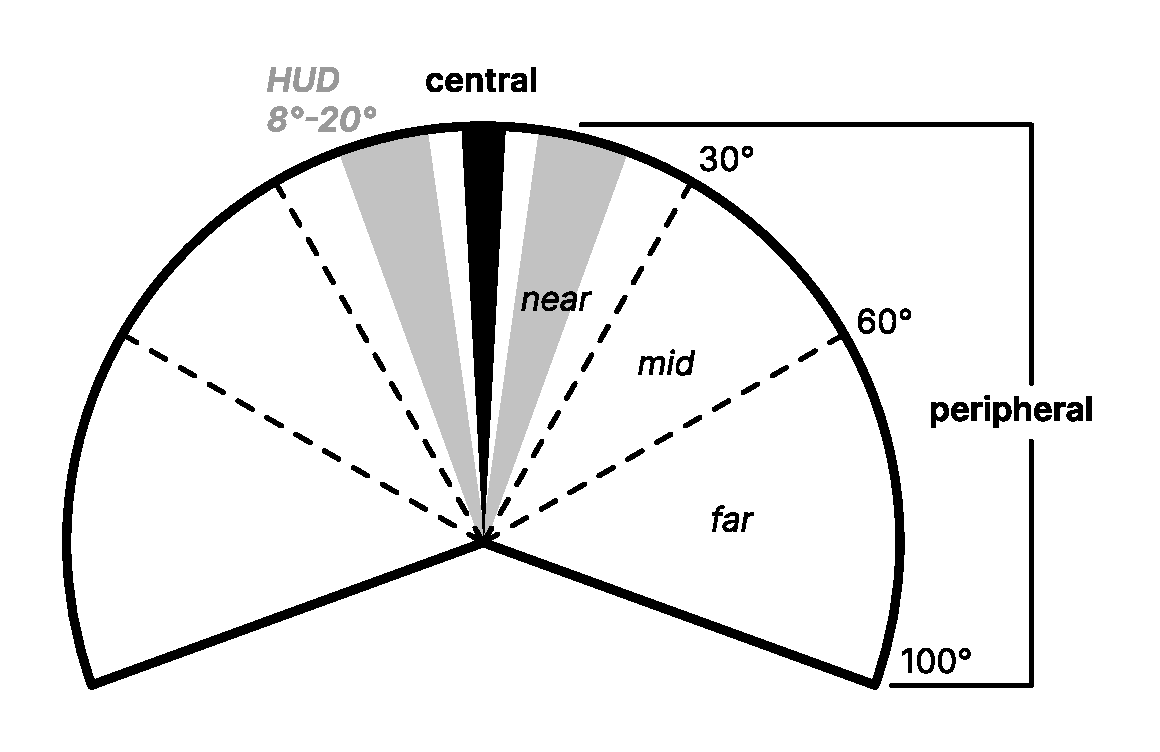
\includegraphics[width=0.5\textwidth]{assets/FOV.eps}
    \caption{Example notification with billboard style.}
    \label{fig:notif}
\end{figure}

The core example of the notification system is the high priority warning. This component is designed with a so-called billboard style, meaning text with a surrounding box. The big, bright area ensures high visibility even if the pop-up is not in the center of vision. Since it is the highest priority, it is the only element placed in the upper part of the screen. To avoid blocking central vision for too long, the pop-up will transform into a smaller version at the upper edge of the screen.

Grabs attention first, readability second step -> text case?
Oxygen vs O2/abbreviations better?

\subsubsection{The Checklist Component}

Since this element is text-based, it relies less on peripheral vision.
To anchor the gaze the current task is centered on the screen and more distinctive than the other displayed tasks.
Though the other tasks are smaller, everything is left-aligned to—once again—create an optical guide.

sentence case vs lower case

Note that this component is meant as a visual example, which is why certain aspects of functionality might not work in regard to handling the list. (e.g. if only two next tasks are displayed, there is no way to see if new tasks got added -> task number display in dynamic situations, generally better for protocol)

The icon to the right is an anchor for possible gaze-based interaction, in this case to show more details. This design keeps the current task centered in the detailed view as well for faster orientation. This also mitigates side effects from possible false positives—i.e. if the system mistakenly opens the detailed view.

\subsection{UI Examples}

\emph{Note: the following illustrations are not to scale.}

The maximum variant of the interface was designed with full functionality in mind, based on Microsoft's HoloLens 2\footnote{}. This includes a horizontal field of view of 43°, a resolution of 1440 by 936 pixel per eye and full color availability (within the technical limits mentioned in section \ref{sec:AR}).

\begin{figure}[hbt]
    \centering
    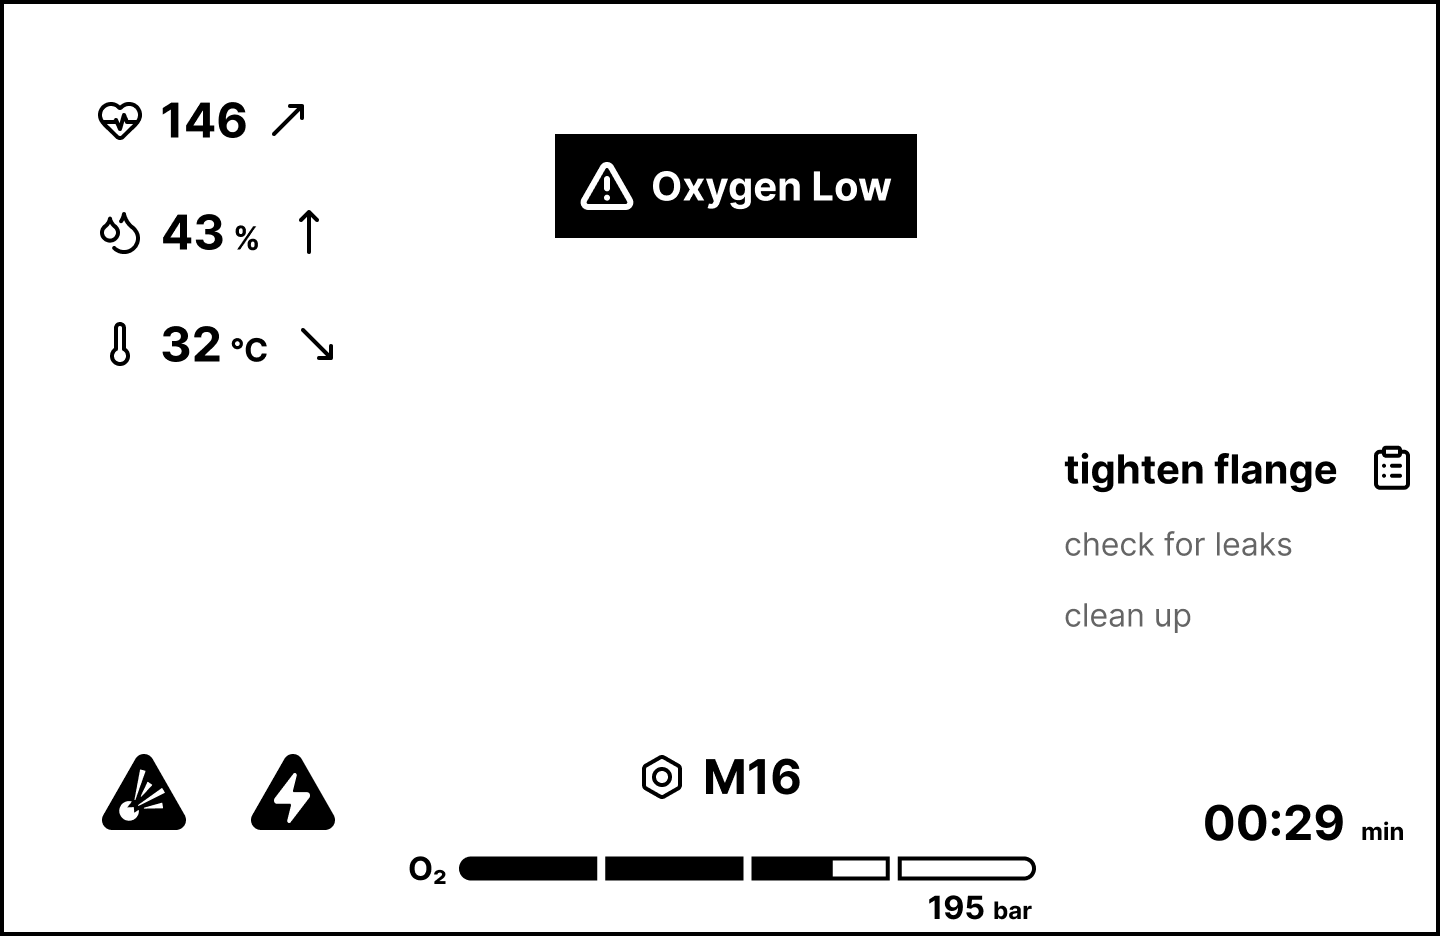
\includegraphics[width=1\textwidth]{assets/UI_max.png}
    \caption{Full-featured UI concept for a binocular HUD.}
    \label{fig:UI_max}
\end{figure}

The layout is based on a three by three grid, anchoring components to the sides and corners, leaving the center free.

While oxygen is the most important element, it is not necessarily the one that is checked the most, but it should be checkable the quickest. -> lower center seems good KATSUYAMA 1989

Occasional information is placed above the oxygen bar, for the same reason: looking down is faster than looking up.

The minimum version is based on the Google Glass, featuring a monocular display with a resolution of 640 by 360 pixels.

https://vr-compare.com/compare?h1=EkSDYv0cW\&h2=EnqtMtA05

A point could be made for overlapping components somewhat to use the space better. However, this would disrupt the grid pattern and optical guides, resulting in longer search times.

\begin{figure}[hbt]
    \centering
    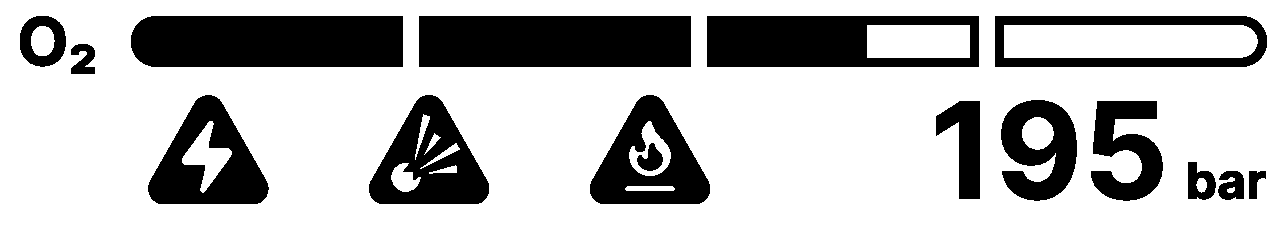
\includegraphics[width=1\textwidth]{assets/UI_overlap.eps}
    \caption{UI concept for a monocular HUD, worn in the upper left of the field of vision.}
    \label{fig:UI_overlap}
\end{figure}

\begin{figure}[hbt]
    \centering
    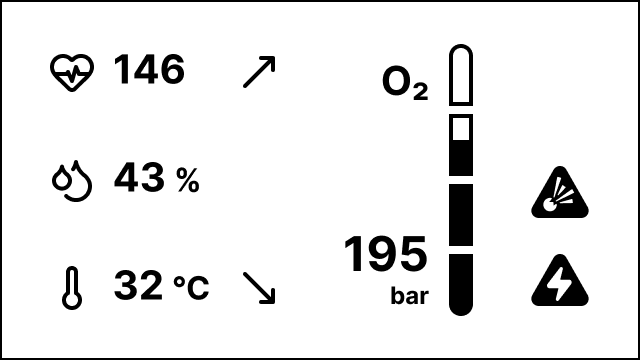
\includegraphics[width=1\textwidth]{assets/UI_min.png}
    \caption{UI concept for a monocular HUD, worn in the upper left of the field of vision.}
    \label{fig:UI_min}
\end{figure}

\begin{figure}[hbt]
    \centering
    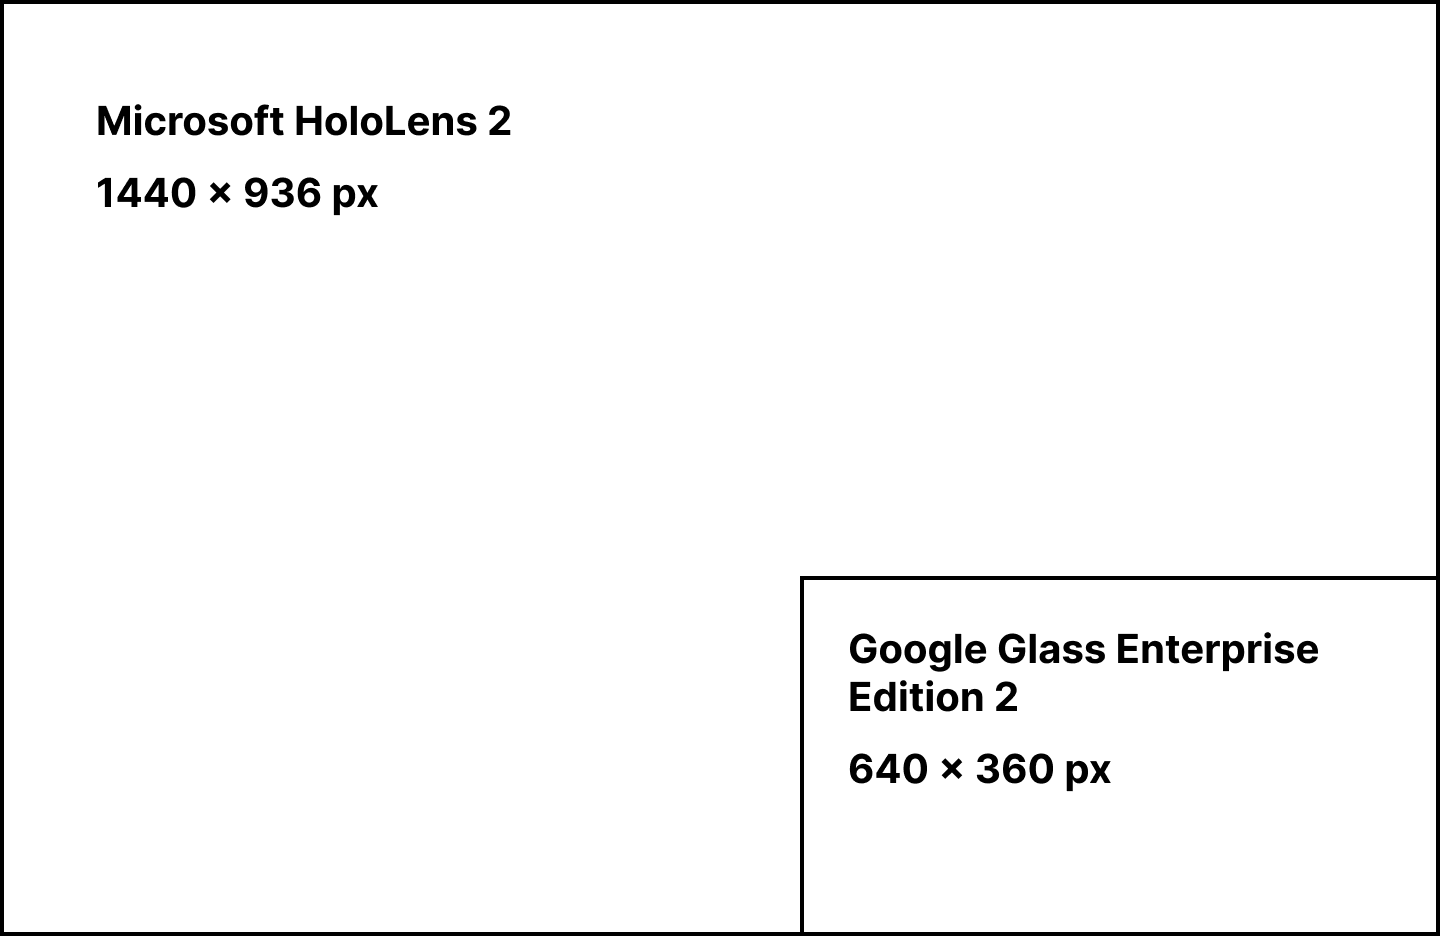
\includegraphics[width=1\textwidth]{assets/HUD_size.png}
    \caption{Size comparison of the Microsoft HoloLens 2 and the Google Glass Enterprise Edition 2.}
    \label{fig:HUD_size}
\end{figure}